\documentclass{article}

\usepackage[utf8]{inputenc} % если ваш файл содержит русский текст, нужно указать кодировку
\usepackage[russian]{babel} % для того, чтобы писать русский текст
\usepackage{amsmath} % для команды equation*
\usepackage{hyperref} % для вставки ссылок
\usepackage{graphicx}
\usepackage{mathtools}

% \usepackage[utf8]{inputenc}
% \usepackage[english]{babel}
 
\usepackage[dvipsnames]{xcolor}

\title{Differential Equations Computational Practicum}
\date{2019-11-14}
\author{Timur Gainullin}


\begin{document}
% \textrm{Sample Text 0123}
	\pagenumbering{gobble} % сейчас будет титульная страницу, отключим нумерацию страниц
	\maketitle % эта команда печатает титульную страницу

	\newpage % эта команда начинает новую страницу
	\pagenumbering{arabic} % включим нумерацию страниц обратно



\section{Introduction}

Given the initial value problem:
\[
	\begin{dcases}
		y' = 1 + 2y / x\\
		y(1) = 2\\
		x \in (1, 10)
	\end{dcases}
\]

Needed to solve it analytically and using 3 numerical methods. Solutions should be analized and compared to each other. To provide data visualization I chose JavaFX and used OOP-design in code structure. Repository is avalible
\href{https://github.com/Tumypmyp/DE_Practicum}{\color{blue}{\underline{here}}}. But firstly lets find exact solution for this equation.


\section{Analytical solution}

	$$y' = 1 + \frac{2y}{x}$$

	$$y' - \frac{2y}{x} = 1$$

A nonhomogeneous equation of form y' + f(x)y = g(x) and can be
solved using the integrating factor:

	$$\mu(x) = e^{\int{\frac{-2}{x} \partial x}} = x^{-2}$$
	$$\frac{\frac{\partial y}{\partial x}}{x^2} - \frac{2y}{x^3} = \frac{1}{x^2}$$
	$$\frac{\frac{\partial y}{\partial x}}{x^2} - \frac{\partial}{\partial x}\left(\frac{1}{x^2}\right)y = \frac{1}{x^2}$$

Apply the reverse product rule:
	$$\frac{\partial}{\partial x}\left(\frac{y}{x^2}\right) = \frac{1}{x^2}$$

Integrate both sides with respect to $x$:
	$$\int{\frac{\partial}{\partial x}\left(\frac{y}{x^2}\right)}\partial x = \int{\frac{1}{x^2}}\partial x$$
	$$ \frac{y}{x^2} = -\frac{1}{x} + c_1$$
	$$y = x(c_1x - 1)$$

Using $y(1) = 2$:

	$$2 = c_1 - 1$$
	$$c_1 = 3$$
The solution is:
	$$y = x(3x - 1), \quad x \neq 0$$

\section{Numerical solutions}

\subsection{Code}
To avoid same code in different \texttt{NumericalMethod}s when we need to calculate local and total errors
I wrote function that updates this graph in \texttt{ExactSolution} class. This is code I got with function 
that just updates solution for comparation: 


\begin{verbatim}
    public void updateXYChart(XYChart.Series series) {
        series.getData().clear();
        for (int i = 0; i < N; ++i) {
            series.getData().add(new XYChart.Data(getKey(i), getValue(i)));
        }
    }

    public void updateLocalErrorXYChart(XYChart.Series series, 
    		NumericalMethod numericalMethod) {
        series.getData().clear();
        for (int i = 0; i < N; ++i) {
            series.getData().add(new XYChart.Data(i, getValue(i)
            	- numericalMethod.getValue(i)));
        }
    }

\end{verbatim}



\subsection{Application}
There is some screenshots of application:
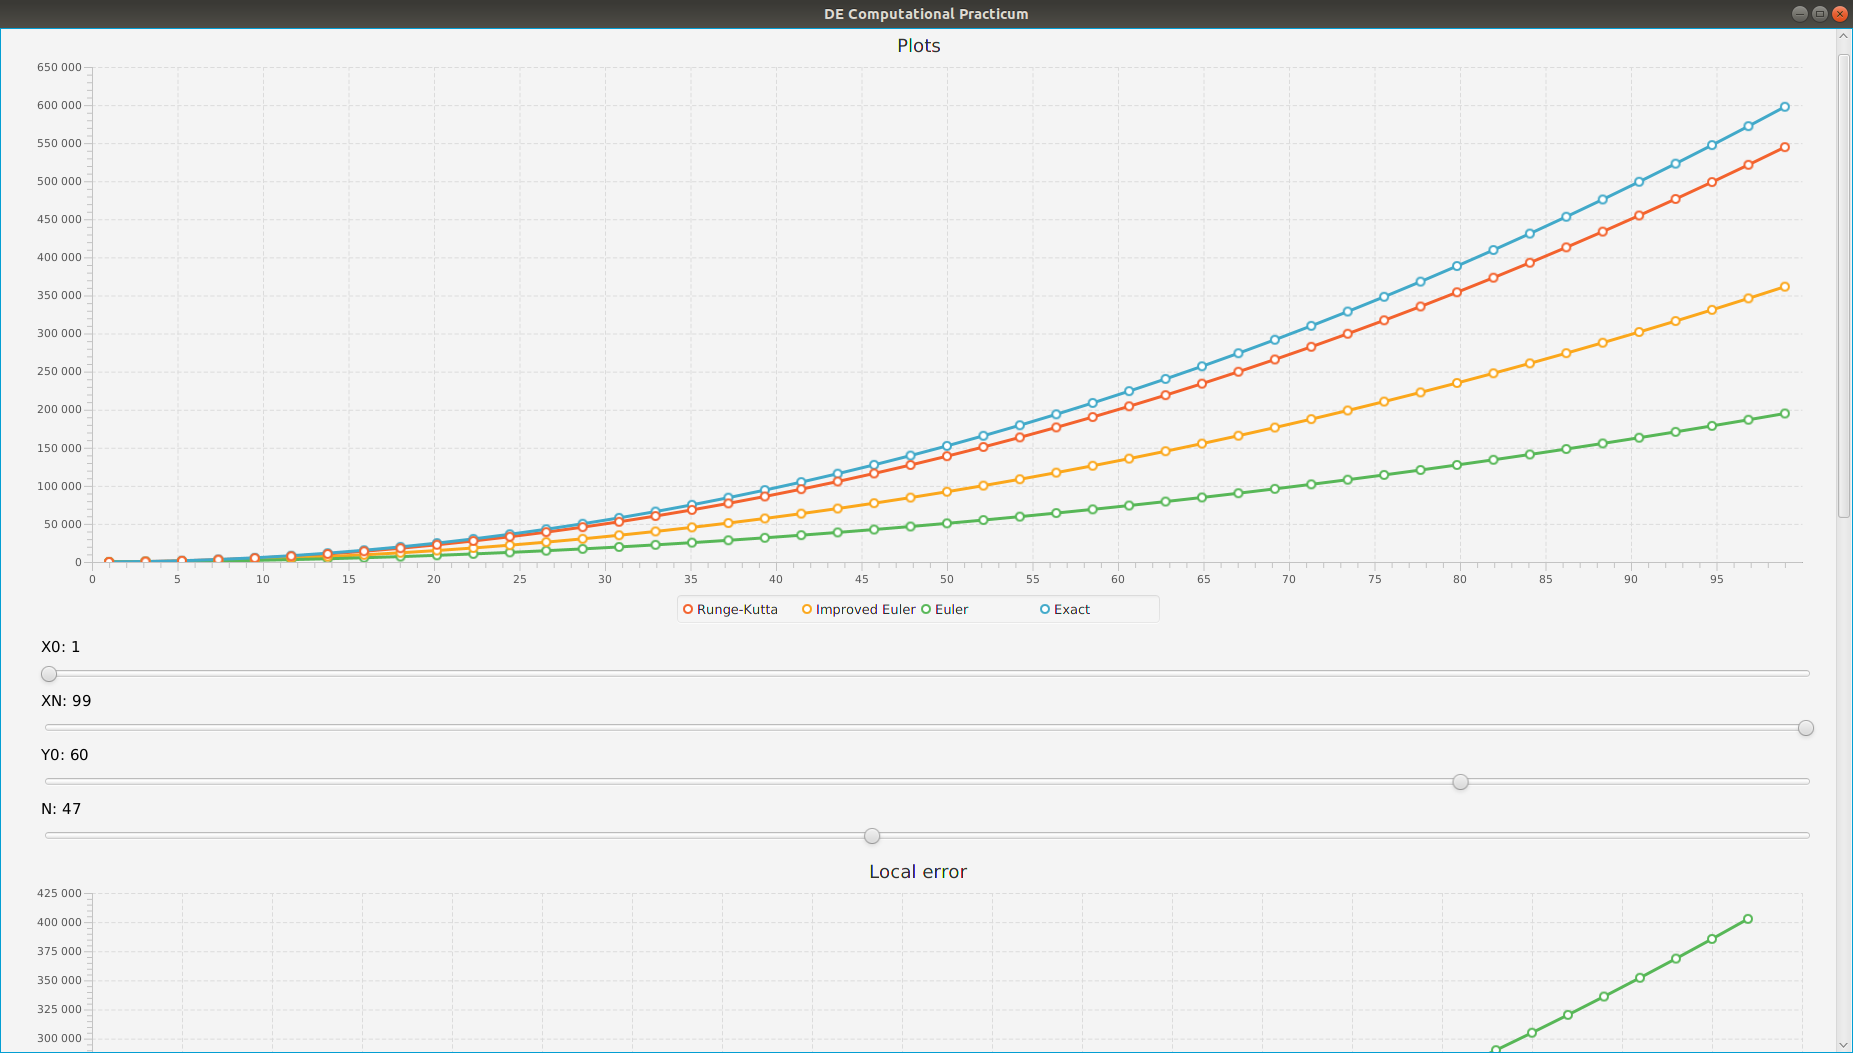
\includegraphics[scale=0.2]{Plots.png}
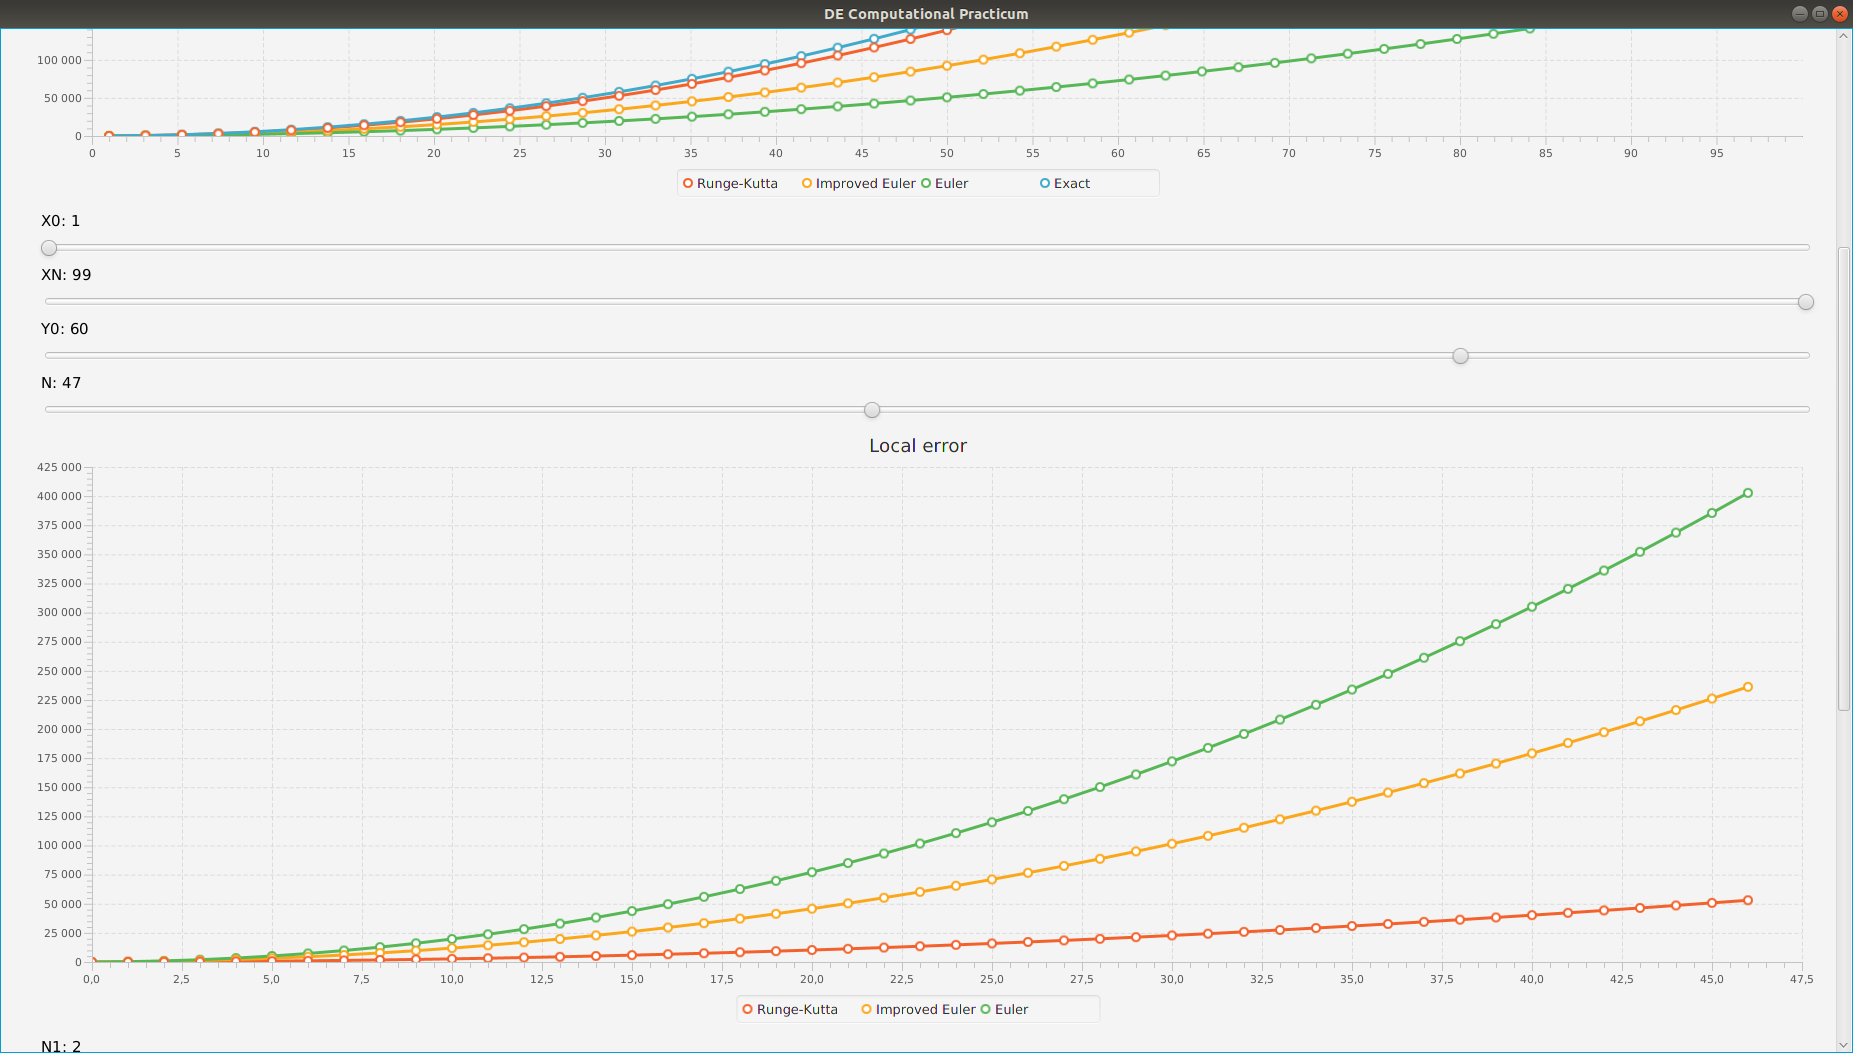
\includegraphics[scale=0.2]{LocalErrors.png}
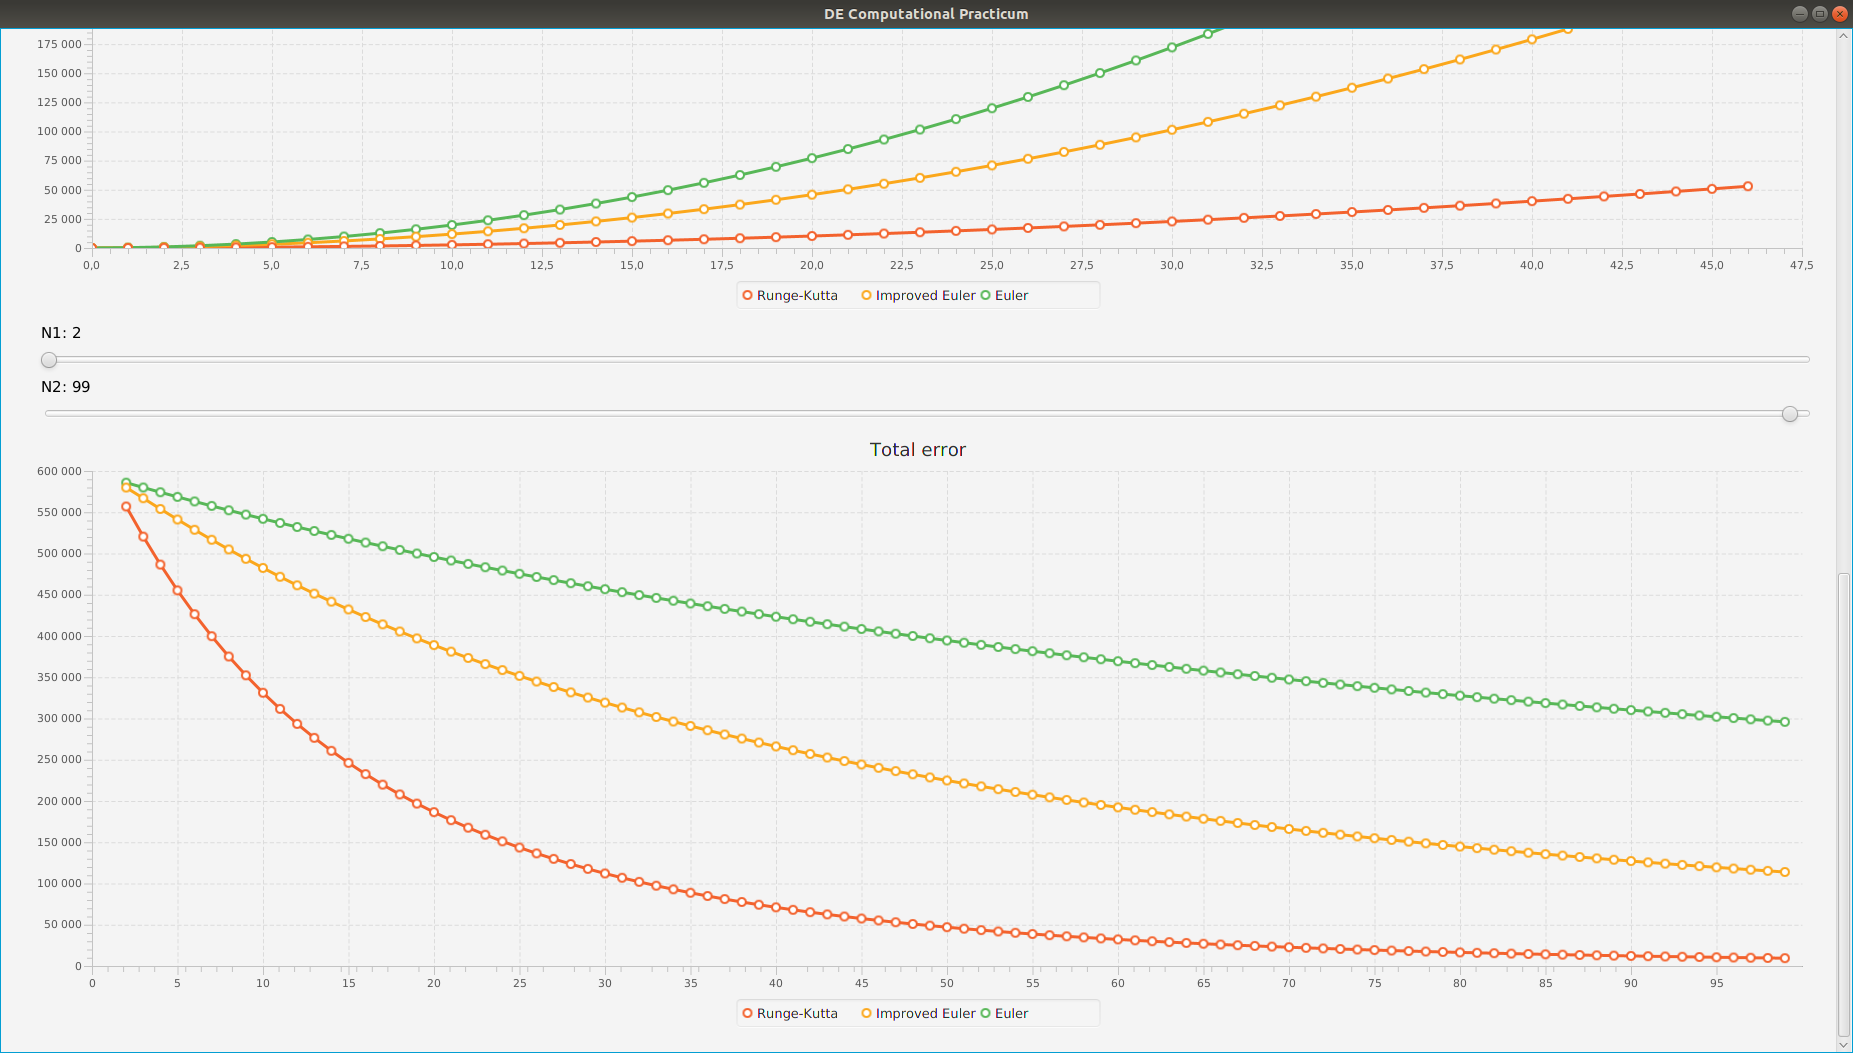
\includegraphics[scale=0.2]{TotalErrors.png}
\subsection{UML-diagram}
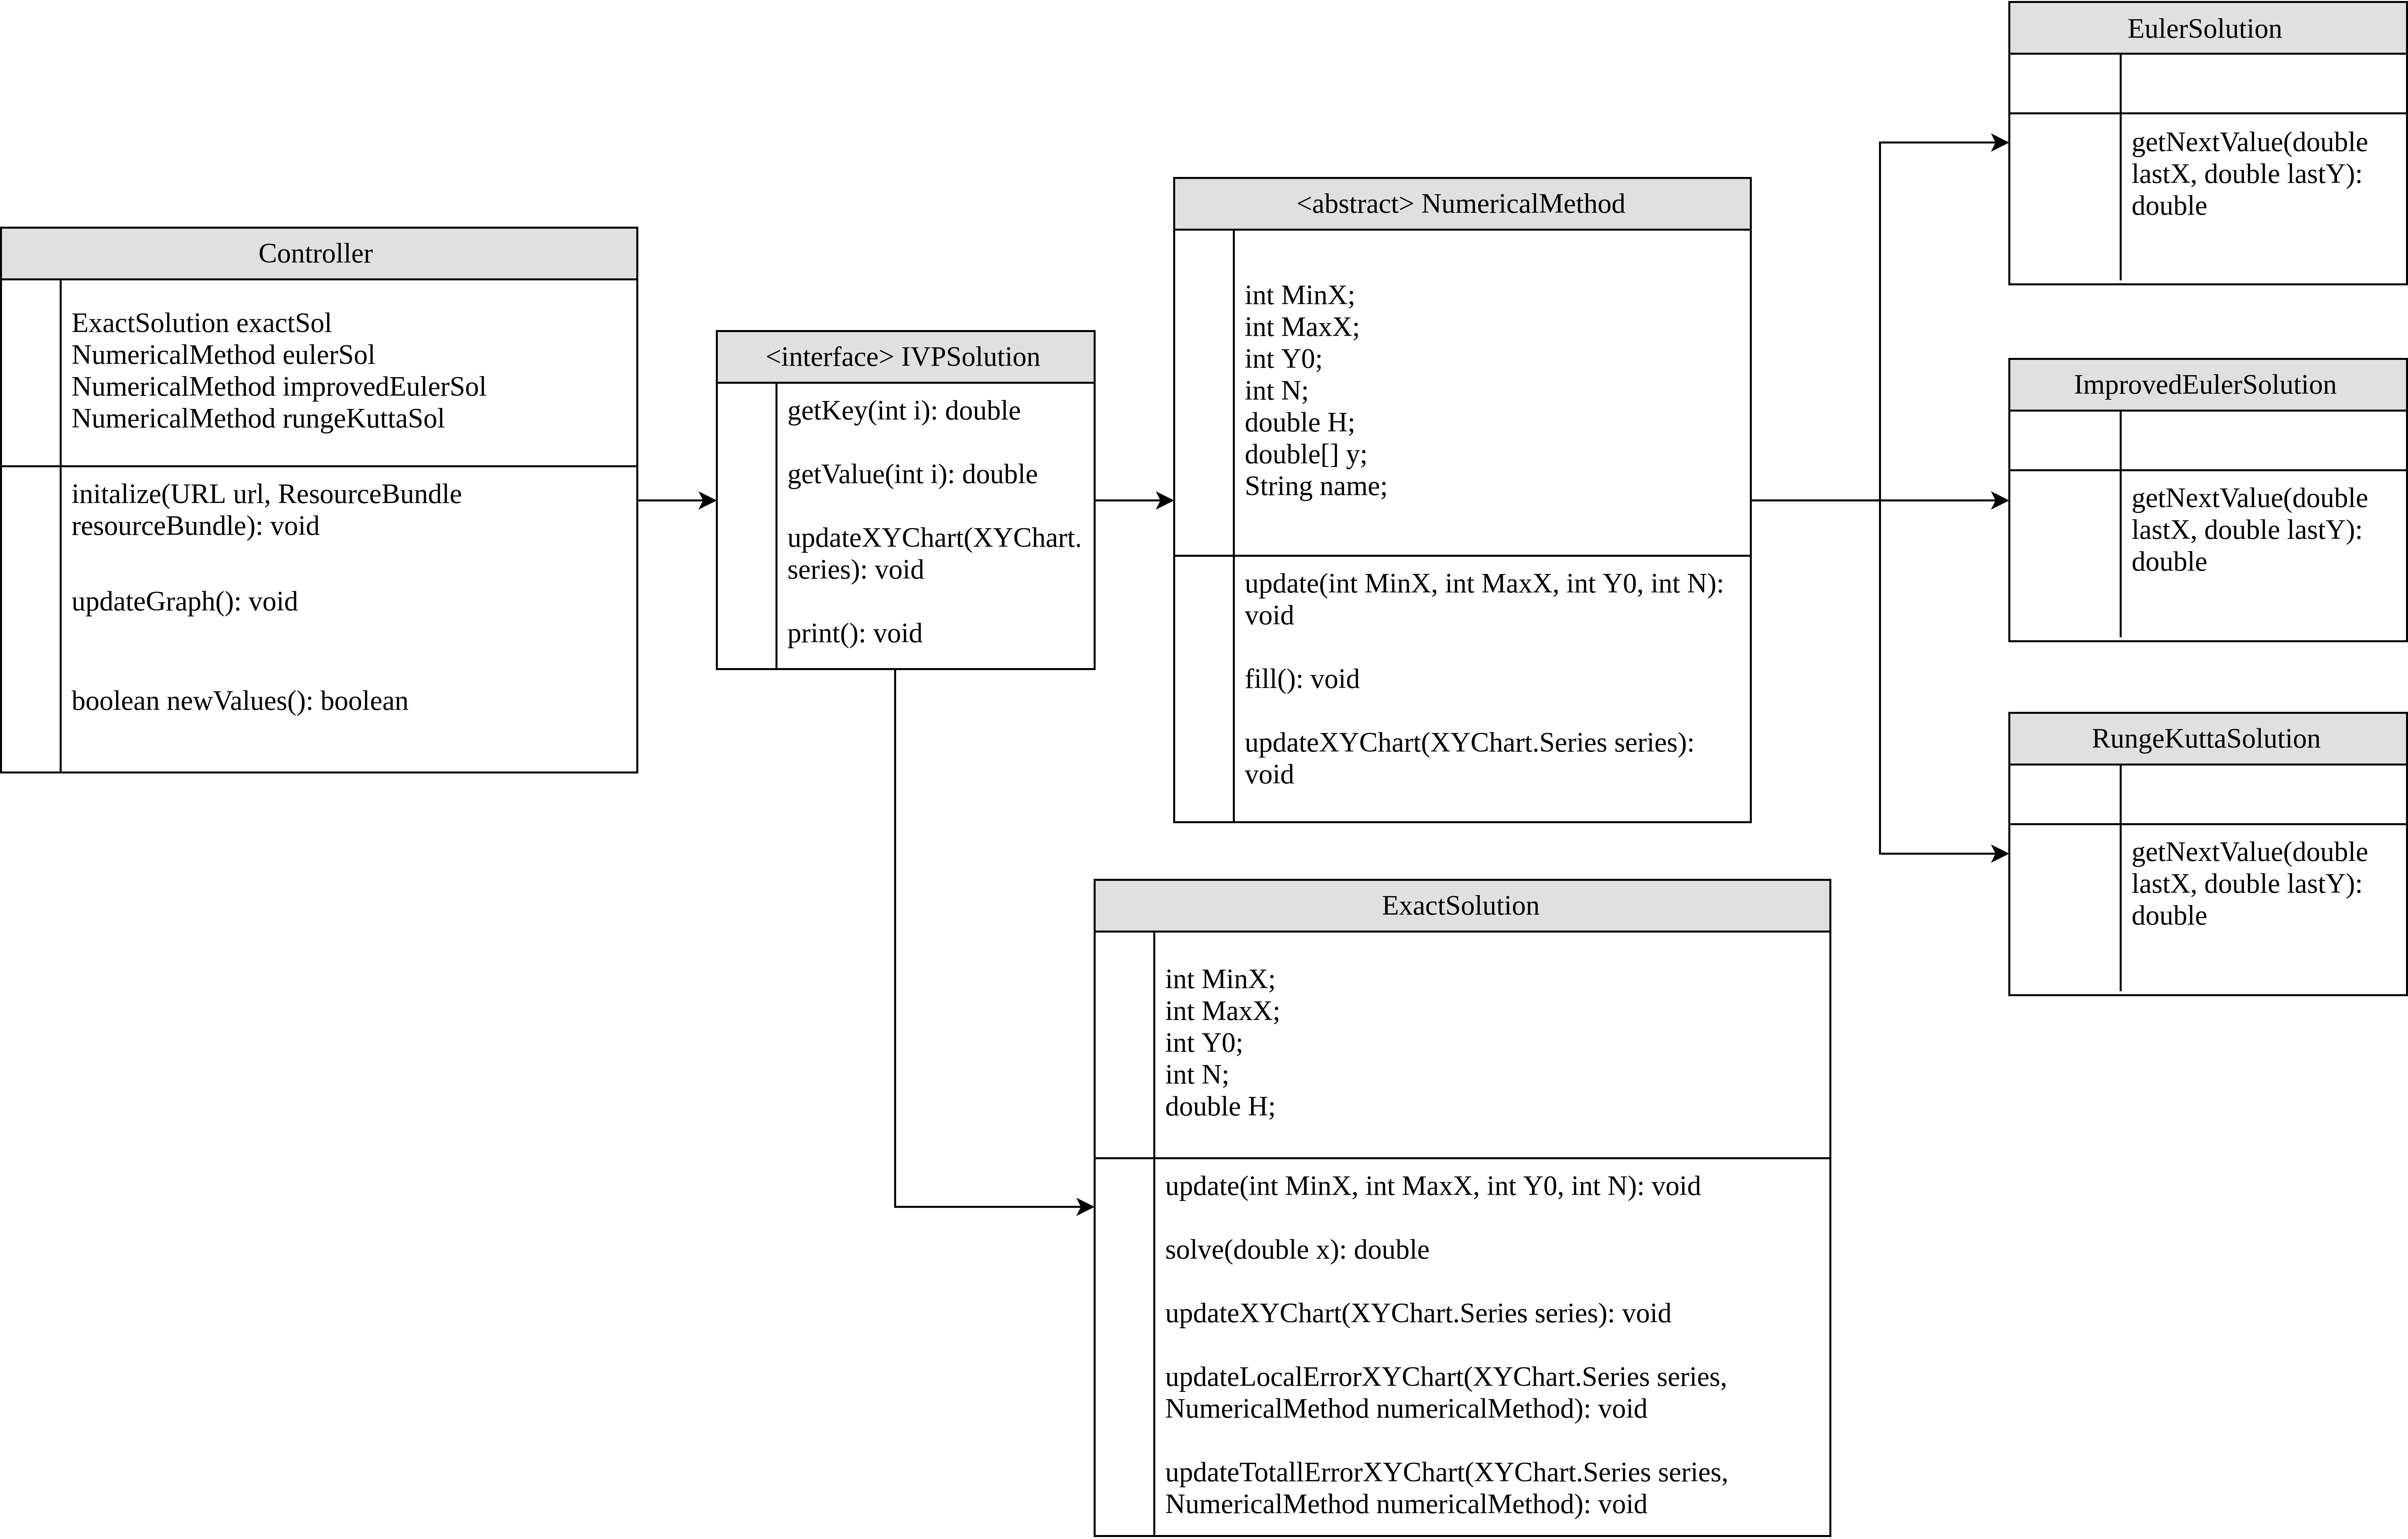
\includegraphics[scale=0.5]{UML.png}

\end{document}